\documentclass[5p,times]{elsarticle}

% The following \documentclass options may be useful:

% preprint      Remove this option only once the paper is in final form.
% 10pt          To set in 10-point type instead of 9-point.
% 11pt          To set in 11-point type instead of 9-point.
% numbers       To obtain numeric citation style instead of author/year.

\usepackage{amsmath}
\usepackage{mathtools}
\usepackage{graphicx}
\usepackage{listings}
\usepackage{color}
\usepackage{xcolor}
\usepackage{amsmath}
\usepackage{semantic}
\usepackage{url}
\usepackage{natbib}
\bibliographystyle{plainnat}
\usepackage[utf8]{inputenc}
\usepackage[english]{babel}
\usepackage{stmaryrd}
\usepackage{pgf}
\usepackage{caption}
\usepackage{subcaption}
\usepackage{multicol}
\usepackage{wasysym}
\usepackage{tikz}
\usepackage{amssymb}
\usepackage{graphicx}
\usepackage{epstopdf}
\usepackage{enumitem}
\usepackage{tocloft}
\usepackage{setspace}

\setlength\cftparskip{-2pt}
\setlength\cftbeforesecskip{1pt}
\setlength\cftaftertoctitleskip{2pt}
\setcounter{tocdepth}{1}

\usetikzlibrary{matrix,arrows,decorations.pathmorphing}

\definecolor{keywords}{rgb}{0,0,200}
\definecolor{comments}{rgb}{0,0.5,0}
\definecolor{types}{rgb}{0.99,0.1,0.99}
\definecolor{strings}{rgb}{0.5,0,0}

\def\figfontsize{\fontsize{6}{7}}

\lstdefinelanguage{ESL}{
         basicstyle=\footnotesize\ttfamily, % Standardschrift
         numbersep=5pt,              % Abstand der Nummern zum Text
         tabsize=1,                  % Groesse von Tabs
         extendedchars=true,         %
         breaklines=true,            % Zeilen werden Umgebrochen
         morecomment=[l]{//},
         columns=fullflexible,
         aboveskip=2mm,
         belowskip=2mm,
         frame=tb,
         stringstyle=\color{strings},
         commentstyle=\color{comments}, % style of comments
         keywordstyle=[1]{\ttfamily\color{keywords}}, 
         keywords=[1]{grab,or,case,for,null,data,if,else,new,type,probably,fun,set,bag,
                       fold,unfold,find,in,when,then,let,not,letrec,act,self,become,export,and},
         keywordstyle=[2]{\ttfamily\color{types}}, 
         keywords=[2]{Act,Int,Bool,Str,Float,Array,Hash,Void,Fun,rec,Set,Bag},
         numbers=left,
         moredelim=[s][\color{strings}]{'}{'},
         moredelim= [s][\color{red}]{/*}{*/},
         escapeinside={(*}{*)},
         literate=%
           {...}{$\ldots$}{1}
           {::}{$\dblcolon$}{1}
           {->}{${\mathbin{\rightarrow}}$}1
           {<-}{$\leftarrow$}{1},
         showspaces=false,           % Leerzeichen anzeigen ?
         keepspaces=true,
         showtabs=false,             % Tabs anzeigen ? 
         showstringspaces=false      % Leerzeichen in Strings anzeigen ?        
 }

\lstnewenvironment{ESL} { \lstset{language=ESL} } { }

\lstnewenvironment{ESL*} { \lstset{language=ESL,frame=none} } { }

\lstnewenvironment{FigESL} { \lstset{language=ESL,frame=none,basicstyle=\figfontsize\ttfamily} } { }
  
\def\code#1{{\normalfont\lstinline[language=ESL,escapeinside={(*}{*)},basicstyle=\footnotesize\ttfamily]{#1}}}

\title{ESL Reference Guide} 

\begin{document}

\maketitle

\tableofcontents

\section{Introduction}

\label{sec:introduction}

This document describes the language ESL and its implementation. ESL is an actor-based language that has been designed to offer a convenient way to build applications that benefit from a large number of independent concurrent processes that communicate in terms of structured data. ESL compiles directly to Java source code and can therefore easily integrate with Java applications. The benefit of using ESL compared to Java is the abstraction that it provides over the construction and management of processes and the data that is passed between them. In addition, ESL enforces a separation of concerns since communication is by asynchronous message which reduces the risks associated with large scale concurrency due to race conditions and shared data. Having said that, whilst ESL actors are encapsulated, it is unreasonable to build a large scale system without some degree of shared data, so ESL provides mechanisms for data sharing where needed. ESL aims to support system verification through an expressive statically checked type system.

\begin{figure}
\centering
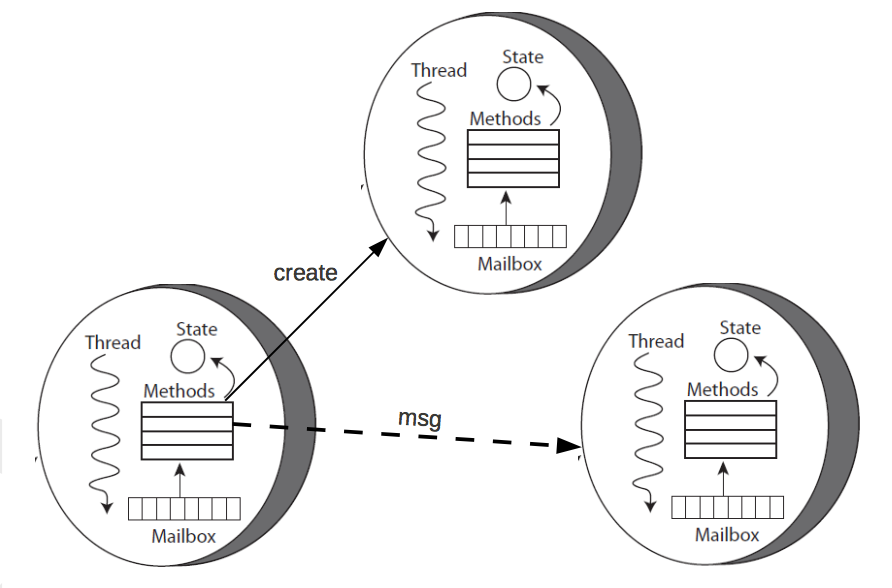
\includegraphics[width=\columnwidth]{actors}
\vspace{-0.20cm}
\caption{Actor Model of Computation \cite{karmani2009actor}}
\label{fig:actors}
\end{figure}

The Actor Model of Computation is characterised in figure \ref{fig:actors} which shows three actors. Each actor has a local thread of control which selects a message from the head of the mailbox and processes it. When the current message is processed, the thread inspects the mailbox for the next message; if no message is available then the actor becomes idle until a message is received. Each actor has a local state that can be inspected and updated by the methods that handle the messages.

An actor can send messages to any actor that it knows about. An actor will know about an actor if it created the actor or it received the actor as part of a message. A message may contain basic data items, collections of data item, actors, and functions. When a source actor passes a function to a target actor, the source may provide access to its internal state when the target calls the function on its own thread.

%%% Motivation for ESL

%%%The Actor Model

%%%Document Guide

\section{Data}

%%% Include lists, comprehensions and builtin operations.
%%% Void.
%%% QSort.
%%% terms and pattern matching.
%%% Equality.

ESL provides basic data types: integers, floats, booleans and strings. For example the following listing declares identifiers along with their values. Comments follow the Java format:
\begin{ESL}
/* The parameters of the program are defined below.
   Change the starting position to get a different
   configuration. */
   
x::Int         = 100;     // Starting x position.
y::Int         = 200;     // Starting y position.
pi::Float      = 3.14;    // Used for position calculation.
isActive::Bool = true;    // True when moving.
name::Str      = 'Wilma'; // Used as a unique identifier.
\end{ESL}
ESL supports homogeneous arrays, for example the following is a one- dimensional array of strings with 100 elements indexed from 0:
\begin{ESL}
names::Array[Str] = new Array[Str](100);
names[0] := 'Wilma';
print[Str]('value at 0 = ' + names[0]);
\end{ESL}
Arrays may be nested, for example to create a two-dimensional array of booleans:
\begin{ESL}
points::Array[Array[Bool]] = new Array[Array[Bool]](100);
for x::Int in 0..100 do {
  points[x] := new Array[Bool](200);
  for y::Int in 0..200 do {
    points[x][y] := true;
  }
}
\end{ESL}
Note that array elements can be updated and passed between actors, therefore they are a basis for race conditions and other concurrency problems. The intention is that arrays are used locally within an actor as efficient indexable storage. If arrays are shared then access should be protected using locks.

ESL provides homogeneous lists whose elements cannot be modified by side effect and are therefore safe to pass between actors. A list is constructed using \code{::} and \code{[ ... ]} and can be decomposed using the operations \code{head} and \code{tail} in addition to pattern matching (see below). For example:
\begin{ESL}
nums::[Int] = [1,2,3,4,5,6,7,8,9,0];
print[Int](head[Int](nums));
print[[Int](tail[Int](nums))
print[[Int]](head[Int](nums) : tail[Int](tail[Int](nums));
\end{ESL}
which produces \code{1}, \code{[2,3,4,5,6,7,8,9,0]} and \code{[1,3,4,5,6,7,8,9,0]} respectively. Note that the operations \code{head} and \code{tail} are supplied with the type of the list element; this is because there operations are {\it polymorphic} as described in section \ref{sec:polymorphism}. The definition of \code{nums} above is equivalent to:
\begin{ESL}
nums::[Int] = 1:2:3:4:5:6:7:8:9:0:[];
\end{ESL}
Sets and bags are like lists except the elements are not ordered. Adding an element to a set or bag produces a new set or bag respectively. Adding an element to a set has no effect if the set already contains the element, otherwise both the set and bag are extended:
\begin{ESL}
setOfNames::Set{Str} = Set{'Fred','Wilma'};
bagOfNames::Bag{Str} = Bag{'Fred','Wilma'};
print[Set{Str}](Set{'Fred' | setOfNames});
print[Bag{Str}](Bag{'Fred' | setOfNames});
\end{ESL}
produces \code{Set\{'Fred','Wilma'\}} and \code{Bag\{'Fred','Wilma','Fred'\}} respectively. Note that extraction from sets and bags occurs via pattern matching is described below.
\begin{figure*}
\centering
\begin{tabular}{|c|c|}
\hline
{\bf Type}&{\bf Equality for Values of Type}\\\hline
\code{i1,i2::Int} & \code{i1} and \code{i2} are the same number\\\hline
\code{f1,f2::Float} & \code{f1} and \code{f2} are the same number\\\hline
\code{s1,s2::Str} & \code{s1} and \code{s2} have the same characters in order\\\hline
\code{b1,b2::Bool} & \code{b1} and \code{b2} are the same boolean values\\\hline
\code{h1:l1,h2:l2::[T]} & \code{h1} is equal to \code{h2}, and \code{l1} is equal to \code{l2}\\\hline
\code{[]::[T]}&equal to an empty list of the same type.\\\hline
\code{set\{e1::T | s1::Set\{T\}\} set\{e2::T | s2::Set\{T\}\}} & \code{e1} and \code{e2} are equal, and \code{s1} and \code{s2} are equal\\\hline
\code{set\{\}::Set\{T\}}&is only equal to an empty set of the same type.\\\hline
\code{bag\{e1::T | b1::Bag\{T\}\} bag\{e2::T | b2::Bag\{T\}\}} & \code{e1} and \code{e2} are equal, and \code{b1} and \code{b2} are equal\\\hline
\code{bag\{\}::Bag\{T\}}&is only equal to an empty bag of the same type.\\\hline
\code{a1,a2::Array[T]} & \code{a1} and \code{a2} are the same array\\\hline
\code{t1,t2::Hash[K,V]} & \code{t1} and \code{t2} are the same table\\\hline
\code{a1,a2::Act \{...\}} & \code{a1} and \code{a2} are the same actor\\\hline
\code{f1,f2::(T ...) -> T} & \code{f1} and \code{f2} are the same function\\\hline
\code{r1,r2::\{ n->T ... \}}& \code{r1.n} is equal to \code{r2.n} for all names\\\hline
\code{C(n1,...), C(m2,...)}& equal when corresponding \code{ni} and \code{mi} are equal\\\hline
\code{null[T]} & only equal to the value null\\\hline
\end{tabular}
\caption{Data Equality}
\label{fig:data_equality}
\end{figure*}
Sets require a definition of equality for ESL values which is provided in figure \ref{fig:data_equality}.

ESL hash tables map keys to values. A hash table provides operations for adding a mapping, accessing the value for a key, testing whether a mapping exists. A hash table uses field reference to get the list of keys and the list of values:
\begin{ESL}
ages::Hash[Str,Int] = new Hash[Str,Int];
ages.put('Fred',35);
ages.put('Wilma',32);
print[Bool](ages.hasKey('Fred'));
print[Int](ages.get('Wilma'));
print[[Str]](ages.keys);
print[[Int]](ages.vals);
\end{ESL}
prints \code{true}, \code{32}, \code{[Fred,Wilma]}, and \code{[35,32]}. Note that because hash tables are updated by side effect, they are not thread safe and should be used locally within an actor, or access should be protected using locks.

ESL functions are first-class values and may be passed between actors within data structures. The rules for identifier binding within functions are defined in section \ref{sec:binding}. A simple example of a function is:
\begin{ESL}
add1::(Int)->Int = fun(x::Int)::Int x + x;
print[Int](add1(100));
\end{ESL}
which prints \code{101}.

Records map names to values. Unlike hash tables, the domain of a record is fixed. New type names can be defined that refer to existing types, so the following code implements an two-dimensional point object:
\begin{ESL}
type Point = { x::Int; y::Int }
mkPoint(n::Int,m::Int)::Point = {x->n; y->m}
print[Point](mkPoint(100,200));
print[Int](mkPoint(100,200).x);
\end{ESL}
prints \code{\{x=100,y=200\}} and \code{100}. Records cannot be updated by side effect.

The value \code{null} can be used as an undefined value for any data type. It is polymorphic and is followed by the type for which it acts as undefined. For example:
\begin{ESL}
x::Int = null[Int];
p::Point = null[Point];
\end{ESL}
The following operations are builtin to ESL:
\begin{ESL}
_ + _     :: (Int,Int)       -> Int
_ + _     :: (Float,Float)   -> Float
_ + _     :: (Str,T)         -> Str
_ + _     :: (T,Str)         -> Str
_ + _     :: ([T],[T])       -> [T]
_ + _     :: (Set{T},Set{T}) -> Set{T}
_ - _     :: (Int,Int)       -> Int
_ - _     :: (Float,Float)   -> Float
_ * _     :: (Int,Int)       -> Int
_ * _     :: (Float,Float)   -> Float
_ / _     :: (Int,Int)       -> Int
_ / _     :: (Float,Float)   -> Float
_ % _     :: (Int,Int)       -> Int
_ = _     :: (T,T)           -> Bool
_ <> _    :: (T,T)           -> Bool
_ and _   :: (Bool,Bool)     -> Bool
_ or _    :: (Bool,Bool)     -> Bool
not       :: (Bool)          -> Bool
print[T]  :: (T)             -> Void
random    :: (Int)           -> Int
wait      :: (Int)           -> Void
isqrt     :: (Int,Int)       -> Float
\end{ESL}

\section{Blocks and Commands}

\label{sec:commands}

The type \code{Void}, like Java, represents an evaluation that does not return a result. The operation \code{print[T](t)} takes a value \code{t::T} and `returns' \code{Void}. A {\it block} is a sequence of {\it commands} enclosed in curly brackets. A command is just any expression, but syntactically, if the expression does not end with a closing \code{\}}, then the command must be terminated with a semicolon. The return value of a block is the return value of the last command. For example:
\begin{ESL}
print3(a::Int,b::Int,c::Int)::Void = {
  print[Int]('first = ' + a);
  print[Int]('second = ' + b);
  print[Int]('third = ' + b);
}
\end{ESL}
The special case of the block \code{\{\}} is of type \code{Void}.

\section{List Comprehensions and List Operations}

\label{sec:cmp}

Lists are a very useful way of organising collections of elements. They can easily be processed using recursion because of their structure: a list is either empty \code{[]} or is a list \code{l} with a head element \code{e} `consed' to the tail: \code{e:l}. 

A {\it list comprehension} is an expression that transforms lists. It has the form: 
\code{[ e | q ... ]}
where \code{e} is an expression and \code{q} is a {\it qualifier}. The idea is that a list is constructed whose elements are formed by evaluating \code{e} after performing each of the qualifiers in turn. There are two types of qualifier: {\it binding} and {\it predicate}. A binding qualifier has the form \code{p <- e} where \code{p} is a pattern and \code{e} is an expression whose value is a list. When it is evaluated, a binding qualifier repeatedly matches the elements from the list against the pattern. A predicate qualifier has the form \code{?e} where \code{e} is a boolean valued expression. When it is evaluated, if the expression in a predicate qualifier produces \code{true} then execution continues, otherwise it ignores the element most recently selected by a binding qualifier and selects the next element. For example:
\begin{ESL}
[ n | n <- 0..100, ?(n % 2 = 0) ]
\end{ESL}
produces a list of even numbers between \code{0} and \code{99} inclusive. Multiple binding qualifiers may be used:
\begin{ESL}
[ mkPoint(x,y) | x <- 0..100, y <- 0..200, ?(x <> y) ]
\end{ESL}
Lists can be processed using recursive functions and pattern matching. Typically a case-expression is used to match against a base case (often \code{[]}) and a recursion case (often \code{h:t}). For example the following operation adds up the distances of all points to the origin:
\begin{ESL}
addDists(ps::[Point])::Float =
  case ps {
    [] -> 0.0;
    h::t -> distanceToOrigin(h) + addDists(t);
  }
\end{ESL}
The following defines Quicksort in ESL:
\begin{ESL}
qsort(l::[Int])::[Int] =
  case l {
    [] ->[];
    x:l ->
      qsort([ n | n <- l, ?(n<x) ])
      + [x] +
      qsort([ n | n <- l, ?(n>x) ]);
  }
\end{ESL}
The collection of list operations that are supported by ESL are shown in \ref{sec:list_operations}.

\section{Algebraic Data Types and Pattern Matching}

ESL supports algebraic data types, also known as {\it union types}. For example, the directions of the compass can be represented using different integers or strings, but it is better to define a new type \code{Direction} and to have 4 unique values of that type. This can be defined as follows:
\begin{ESL}
data Direction =
  North
| South
| East
| West;
\end{ESL}
Now any identifier defined to have type \code{Direction} can hold one of the 4 values and the special value \code{null[Direction]}:
\begin{ESL}
d::Direction = North;
\end{ESL}
Pattern matching can be used with such a data type:
\begin{ESL}
moveRight(dir::Direction)::Direction =
  case dir {
    North -> East;
    East  -> South;
    South -> West;
    West  -> North;
  }
\end{ESL}
Given a list of such directions, they can be mapped:
\begin{ESL}
dirs::[Direction] = [ North, South, East, West ];
[ moveRight(d) | d <- dirs ]
\end{ESL}
The element types of a union can have components. For example a tree of integers:
\begin{ESL}
data TreeOfInt = 
  Branch(TreeOfInt,TreeOfInt)
| Leaf(Int);
\end{ESL}
Note that a branch term contains two integer trees and a leaf contains an integer. The integers in the tree can be added together:
\begin{ESL}
addTreeOfInt(t::TreeOfInt)::Int =
  case t {
    Branch(l,r) -> addTreeOfInt(l) + addTreeOfInt(r);
    Leaf(n)     -> n;
  }
print[Int](addTreeOfInt(Branch(Leaf(100),Leaf(200))));
\end{ESL}
Prints \code{300}. When pattern matching, the case arms are tried in turn, so we can define a short-cut version:
\begin{ESL}
addTreeOfInt(t::TreeOfInt)::Int =
  case t {
    Branch(Leaf(0),t) -> addTreeOfInt(t);
    Branch(t,Leaf(0)) -> addTreeOfInt(t);
    Branch(l,r)       -> addTreeOfInt(l) + addTreeOfInt(r);
    Leaf(n)           -> n;
  }
\end{ESL}
Case arms may contain conditions. For example, adding up all those elements of a tree that satisfy a predicate:
\begin{ESL}
addIf(p::(Int)->Bool,t::TreeOfInt)::Int =
  case t {
    Branch(l,r)       -> addIf(p,l) + addIf(p,r);
    Leaf(n) when p(n) -> n;
    Leaf(n)           -> 0;
  }
addIf(fun(n::Int)::Bool n > 100,Branch(Leaf(100),Leaf(200)));
\end{ESL}
Prints \code{200}.

\section{Sets and Collection Matching}

\label{sec:sets}

ESL supports homogenous sets: the empty set \code{set\{\}}; a set constructed from an element \code{e} and a set \code{s}, \code{set\{e | s\}}; a set union \code{s1 + s2}. Both sets and lists can be processed using pattern matching. For example:
\begin{ESL}
setContainsInt(s::Set{Int},x::Int)::Bool =
  case s {
    set{y | z} when x = y -> true;
    s                     -> false;
  }
\end{ESL}
The operation \code{setContainsInt} uses pattern matching to select the element \code{y} which is equal to the argument \code{x}. Note that sets are unordered, so the pattern \code{set\{y | z\}} is {\it non-deterministic}. When  the supplied value \code{s} matches the pattern, one of the elements in the set is matched against \code{y}; if the pattern fails to match before the corresponding \code{->} then a different element \code{y} will be chosen. In the example, the condition \code{x = y} is within the scope fo the choice, this causes elements from the set \code{s} to be tried un turn until one that matches \code{x} is found or the set is exhausted. If all the values have been tried from the set \code{s} then the case-arm fails and the next case-arm is tried.

Non-deterministic choice may occur more than once in the same pattern. For example, the following returns a duplicate entry in two sets:
\begin{ESL}
duplicate(s1::Set{Int},s2::Set{Int},notFound::Int)::Int =
  case s1,s2 {
    set{x | p}, set{y | q} when x = y -> x;
    s1,s2                             -> notFound;
  }
\end{ESL} 
The first case-arm in \code{duplicate} selects an element \code{x} from \code{s1}, then selects \code{y} from \code{s2} such that they are equal elements. If there is no element in common then the \code{notFound} element is returned.

Non-deterministic pattern-based choice can be used over lists using the pattern \code{p1 + [p2] + p3} where \code{p1} matches a prefix of a list, \code{p2} matches some element, and \code{p3} matches a suffix. The pattern fails in the case that the list if empty. For example, testing whether a given element occurs in a list:
\begin{ESL}
intMember(n::Int,l::[Int])::Bool =
  case l {
    l1 + [x] + l2 when x = n -> true;
    l                        -> false;
  }
\end{ESL}

\section{Actors}

%%% Behaviour types, behaviours, new.

Actors are implemented in terms of {\it behaviour types} and {\it behaviours}. A behaviour type provides an interface definition for a set of behaviours. An interface consists of message types and exported identifiers and their types. Consider a simple behaviour type called \code{Sink} that accepts a single type of message \code{M(Int)}:
\begin{ESL}
Act Sink {
  M(Int);
}
\end{ESL}
Any behaviour of type \code{Sink} must implement the message \code{M}:
\begin{ESL}
act sink::Sink {
  M(n::Int) -> print[Str]('got: ' + n);
}
\end{ESL}
There can be any number of behaviours with the same type:
\begin{ESL}
act sink2::Sink {
  M(n::Int) -> {} // Ignore the message.
}
\end{ESL}
An actor is created with a specific behaviour:
\begin{ESL}
s::Sink = new sink;
\end{ESL}
Once created, the actor can receive messages. A message is asynchronous: \code{s <- M(100)} and is placed on the input queue of the target actor. Each actor is processing at most one message at any time, and is idle if there are no messages on its queue and it is not currently handling a message. Since all actors run concurrently, there is no guarantee that of message ordering other than messages sent from the same actor will retain the ordering in which they are sent.

Any number of behaviours can be defined to conform to a behaviour type. The following shows three different implementations of the type \code{A}. The first, \code{a}, just loops indefinitely which an actor can do because all message handling occurs concurrently with other actors. The second, \code{forward} is supplied with a second actor of type \code{A} to which it forwards messages. Finally, \code{broadcast} is supplied with a collection of actors of type \code{A} and will send any message to all of them:
\begin{ESL}
Act A {
  M(Int,Bool);
}

act a::A {
  M(n::Int,b::Bool) -> 
   self <- M(n,not(b));
}

actor::A = new a;

act forward(other::A)::A {
  M(n::Int,b::Bool) -> 
    other <- M(n,b);
}

proxy::A = new forward(actor);

act broadcast(as::[A])::A { 
  toAll(l::[A],n::Int,b::Bool)::Void =
    case l {
      [] -> {};
      h::A:t::[A] -> {
        h <- M(n,b);
        toAll(t,n,b);
      }
    }
  M(n::Int,b::Bool) ->
    toAll(as,n,b);
  } 

spray::A = new broadcast([new forward(new a) | i <- 0.1000]);

\end{ESL}

Often we want to do some initialisation when an actor is created. The special message handler \code{->} is run each time a new actor is created before any messages are processed:
\begin{ESL}
act sink3::Sink {
  -> print[Str]('I am initialising');
  M(n::Int) -> print[Str]('got: ' + n);
}
\end{ESL}
Actors can refer to other actors. The following pair of actors will bounce messages back and forth until the counter runs down:
\begin{ESL}
Act Ping {
  Ping(Int,Pong);
}

Act Pong {
  Pong(Int,Ping);
}

act ping::Ping {
  Ping(0,p::Pong)      -> print[Str]('stop');
  Ping(n::Int,p::Pong)  -> 
    p <- Pong(n-1,self);
}

act pong::Pong {
  Pong(0,p::Ping)      -> print[Str]('stop');
  Pong(n::Int,p::Ping)  -> 
    p <- Ping(n-1,self);
}

p1::Ping = new ping;
p2::Pong = new pong;
p1 <- ping(100,p2);
\end{ESL}
Behaviour definitions can be parameterised so that new actors can initialise the behaviour. For example, in order to provide an identifier to each actor. In the following example, we create a collection of machines and then broadcast jobs. A machine can process a job if the identifier matches:
\begin{ESL}
Act Machine {
  Process(Int);
}

act machine(id::Int)::Machine {
  Process(m::Int) when m = id -> {
    print[Str]('handling job');
  }
  Process(m::Int) -> {} // Ignore job if not target machine.
}

noOfMs::Int         = 100;
noOfJs::Int         = 10000;
machines::[Machine] = [ new machine(n) | n <- 0..noOfMs ];

for job::Int in 0..noOfJs do {
  let targetMachine::Int = random(noOfMs);
  in {
    for m::Machine in machines do {
      m <- Perform(targetMachine);
    }
  }
}
\end{ESL}
An actor may perform \code{become} to change behaviour. The replacement behaviour must implement the same behaviour type. Subsequent messages are handled by the new behaviour. For example, a resource manager allocates resource on request and becomes pending resource manager for the period of time when resources are unavialable:
\begin{ESL}
type Resource = ...;
Act Consumer {
  Receive(Resource);
}

Act ResourceManager {
  Allocate(Consumer);
  Free(Resource);
}

act manager(rs::[Resource])::ResourceManager {
  Allocate(c::Consumer) when rs = [] -> {
    become pending;
    self <- Allocate(c);
  }
  Allocate(c::Consumer) -> {
    become manager(tail[Resource](rs));
    c <- Receive(head[Resource](rs);
  }
  Free(r::Resource) -> become manager(r:rs);
}

act pending::ResourceManager {
  Allocate(c::Customer) -> self <- Allocate(c);
  Free(r::Resource) -> become manager([r]);
}
\end{ESL}

\section{Binding and Scope}

\label{sec:binding}

%%% Let , letrec, functions, locals in behaviours, state, update, functions. Loops.

ESL is a statically scoped language meaning that identifiers can be referenced within the textual binding block in which they are defined. Identifiers can be introduced as: function arguments; let-bindings; letrec-bindings; behaviour definitions; behaviour arguments (equivalent to function arguments); top-level definitions; pattern variables; for-loop controls. This section addresses each of these categories in turn.

Let-expressions introduce local bindings for the scope of the body of the let. A let-expression may have multiple bindings in which case they are performed in parallel:
\begin{ESL}
let dx::Int = x1-x2;
    dy::Int = y1-y2;
in isqrt((dx*dx)+(dy*dy));
\end{ESL}
A let-binding can be used to define a local function. Special syntax allows a function to be defined without using the keyword \code{fun}:
\begin{ESL}
let 
  distance(x1::Int,y1::Int,x2::Int,y2::Int)::Float =
    let dx::Int = x1-x2;
        dy::Int = y1-y2;
    in isqrt((dx*dx)+(dy*dy));
in distance(100,200,50,70);
\end{ESL}
A letrec-expression can be used to create local recursive functions:
\begin{ESL}
letrec 
  contains(l::[Int],n::Int)::Bool =
    case l {
      [] -> false;
      h:t when h=n -> true;
      h:t -> contains(t,n);
    }
in contains([1,2,3,4,5,6,7,8,9],5);
\end{ESL}
A letrec-expression can be used to create mutually recursive function definitions:
\begin{ESL}
letrec
  isEvan(n::Int)::Bool = if n = 0 then true else isOdd(n-1);
  isOdd(n::Int)::Bool = if n = 0 then false else isEven(n-1);
in isEven(101);
\end{ESL}
Letrec-bindings that do not establish functions are performed in sequence.

Behaviour definitions contain a collection of bindings that are established as a letrec and scoped over the message handlers of the behaviour. In addition, the names of local bindings can be exported and referenced using the \code{_._} operation. An an example, support we have a post office actor that delivers letters to people by matching up the address in the message:
\begin{ESL}
Act Person {
  export getAddress::()->Str;
}

act person(address::Str)::Person {
  export getAddress;
  getAddress()::Str = address;
  Open(Letter);
}

data Letter = Letter(Str,Str);

Act PostOffice {
  Deliver(Str);
}

act postOffice(people::[Person])::PostOffice {
  findPerson(address::Str,people::[Person])::Person =
    case people {
      [] -> throw[Person]('cannot deliver to ' + address);
      p:ps when p.getAddress() = address -> p;
      p:ps -> findPerson(address,people);
    }
  Deliver(Letter(name,address)) -> 
    findPerson(address) <- Open(Letter(name,address));
}
\end{ESL}

\section{Modules}

label{sec:modules}

ESL is a compiled language. The units of compilation are called modules and are usually contained in text files. A module contains a collection of mutually recursive bindings for types, behaviours, functions and values. A module \code{m} may export some of its bindings so that they can be used by any other module that imports \code{m}. For example a module defined in a file \code{a/b/c.esl} defines two names and exports one of them:
\begin{ESL}
export f;

f(n::Int)::Int = g(n) + 1;
g(n::Int)::Int = n + 100;
\end{ESL}
A second module can then import \code{c} and use the exported name:
\begin{ESL}
export main;

import 'a/b/c.esl';

g(n::Int)::Int = n = 200;

act Main::Act{} {
  -> print[Int](f(10));
}
\end{ESL}
prints 111. Note that the second module above defines a behaviour names \code{main}. When building an application there should be a root module that defines \code{main} which is the entry point for the application. When ESL starts to run a module it creates a single actor with the behaviour \code{main}. There is no restriction on the behaviour type of \code{main}.

\section{Time}

\label{sec:time}

ESL applications can be driven by a system clock. This can be useful when the application is driven by click ticks or when the application should run for a specific length of time. In order to receive clock ticks, a behaviour must implement at least one message handler of type \code{Time(Int)}. Any actor with such a behaviour will receive clock ticks {\it when the actor is idle}. If an actor does not define a handler for \code{Time{Int}} then there is no overhead for handling time.

The value of \code{n} in \code{Time(n)} is the time in milliseconds since the start of the application. The frequency of the ticks is undefined and therefore there is no guarantee that an actor will receive a tick with a specific value of \code{n}, and it may be the case the an actor receives multiple messages with the same value of \code{n}.

An actor may call \code{wait(n)} which causes the actor's thread to wait for \code{n} milliseconds. Since all actors have concurrent behaviours, a call of \code{wait} will not affect any other actor.

The following definition shows a typical pattern involving click ticks: two message handlers are defined, the first to detect whether a limit has been achieved and stops the application, the second just ignores the click:
\begin{ESL}
Time(n::Int) when n > limit -> stopAll();
Time(n::Int)                -> {}
\end{ESL}

\section{State}

\label{sec:state}

%%% Shared and grab. Note not needed.

A value binding establishes an association between an identifier and a value. The association has a scope that defines the ESL code where the identifier can be referenced. ESL uses {\it lexical scoping} where the association is established in a construct (module, behaviour, let, letrec, function, case-arm, message handler) whose textual definition is the scope.

The original definition of the actor model of computation does not support side-effects. This restriction provides a rather austere application development platform where certain obvious implementation approaches become more unwieldy than they might otherwise be. Therefore, ESL provides side-effects on value bindings. These must be used with care since the actor model was originally designed to avoid issues such as race conditions that occur because of shared state.

Side-effects may be used to provide actors with mutable state:
\begin{ESL}
Act BankAccount {
  Deposit(Int);
}

act account::BankAccount {
  funds::Int = 0;
  Deposit(n::Int) -> funds := funds + n;
} 
\end{ESL}
An actor may encapsulate its state. Since an actor is singly-threaded, this means that there can be no doubt regarding whether an update has occurred or not when the value of a state variable is used, {\it i.e.} the state is not used by multiple threads. However, it is often useful for an actor to provide access to its internal state via its interface. This can be achieved in one of two key ways: message passing or an interface operation. 

If access is provided by message passing then reference to the state remains singly threaded, however the message must contain the requesting actor who receives the state value via a return message:
\begin{ESL}
Act BankAccount {
  Deposit(Int);
  Withdraw(Int,A);
}

act account::BankAccount {
  funds::Int = 0;
  Deposit(n::Int) -> funds := funds + n;
  Withdraw(n::Int,a::A) when n >= funds -> {
    funds := funds - n;
    A <- Withdrawn;
  }
  Withdraw(n::Int,a::A) -> 
    a <- WithdrawFailed;
} 
\end{ESL}
Alternatively, access may be provided via an interface operation. In this case the state can be accessed using multiple threads raising the possibility of race conditions. Consider the following version of the bank account:

\begin{ESL}
Act BankAccount {
  export 
    getFunds::() -> Int; 
    widthdraw::(Int) -> Void; 
    deposit::(Int) -> Void;
}

act account::BankAccount {
  export getFunds,withdraw,deposit;
  funds::Int = 0;
  getFunds()::Int = funds;
  deposit(n::Int)::Void = funds := funds + n;
  withdraw(n::Int)::Void = 
    if n >= funds 
    then funds := funds - n; 
    else {}
} 
\end{ESL}
Two different actors may share access to a bank account. The first actor performs the following:
\begin{ESL}
a.deposit(100);
a.withdraw(10);
print[Str]('funds = ' + a.getFunds());
\end{ESL}
what value will be printed? We might expect the funds to be increased by \code{90}. However, the answer depends on whether the second actor has performed a deposit or withdrawal in between line \code{1} and \code{2} or between line \code{2} and \code{3}. 

In order to be sure, such transactional blocks must be protected. All access to shared state must use locks to gain exclusive access. Each actor that uses the exported operations must do so within a \code{grab(lock)} block. Any value may be used as the lock providing the same value is used by all threads that share the state. In this case it makes sense to use the account as the lock:
\begin{ESL}
grab(a) {
  a.deposit(100);
  a.withdraw(10);
  print[Str]('funds = ' + a.getFunds());
}
\end{ESL}
Now providing that all actors that share the account use a similar \code{grab(a)} to wrap any transactions, the actor above can be sure that the funds will have been increased by \code{90}.

The scheme above relies on the client actors being well behaved in their use of the bank account by wrapping transactions in a \code{grab(a)}. A better way is for the bank account to enforce the protection of the state whilst still offering an interface. This can be achieved by passing the account a transaction function as follows:
\begin{ESL}
Act BankAccount {
  export 
    transaction::(()->Int,(Int)->Void,(Int)->Void)->Void
}

act account::BankAccount {
  export transaction;
  funds::Int = 0;
  getFunds()::Int = funds;
  deposit(n::Int)::Void = funds := funds + n;
  withdraw(n::Int)::Void = 
    if n >= funds 
    then funds := funds - n; 
    else {}
  transaction(action::(()    -> Int,
                       (Int) -> Void,
                       (Int) -> Void) -> Void)::Void =
    grab(self) {
      action(getFunds,deposit,withdraw);
    }
}
\end{ESL}
Any client actor must provide the account with an action which is performed on the client's thread and is guaranteed to occur within the scope of the lock:
\begin{ESL}
a.transaction(fun(getFunds::()    -> Int,
                  deposit::(Int)  -> Void, 
                  withdraw::(Int) -> Int)::Void {
  deposit(100);
  withdraw(10);
  print[Str]('funds = ' + getFunds());
});
\end{ESL}

\section{Concurrency}

\label{sec:concurrency}

ESL actors run concurrently. An actor is created using \code{new b} or \code{new b(x,...)} which immediately returns a handle to the newly created actor and schedules the thread of the newly created actor. The behaviour \code{b} may have an initialisation clause (a message handler starting with \code{->}) that is the first action performed on the new thread. After initialisation, the new thread enters a loop that inspects the actor's message queue and dispatches to a message handler in \code{b} if a message exists, otherwise the thread waits until a message is received. If \code{b} defines a handler for \code{Time(Int)} then the ESL system sends the actor a message providing the queue is empty.

ESL is designed to make the creation and interaction of concurrent actors very lightweight. As described in \code{sec:state}, actors can share state and, if so, must make appropriate use of locks. However, in general the state of an actor is encapsulated and is modified by third party actors using message passing. 

The use of large scale concurrency and asynchronous message passing changes the conventional approach to system design and implementation which is based on task decomposition and sequential ordering. This section provides a number of examples that show how actors can be used to implement tasks that take advantage of the concurrent computational model.

\subsection{Search}

\label{sec:search}

\begin{figure}[t]
\begin{ESL}
Act Main       {                   } 
Act Searcher   { Time(Int);        }   
Act Controller { Time(Int); Found; }   

size::Int                = 1000;                          
numOfSearchers::Int      = 10;                            
board::Array[Array[Str]] = new Array[Array[Str]](size);   
max(a::Int,b::Int)::Int  = if a > b then a; else b;      

act controller::Controller {
  count::Int = 0;                              
  Time(n::Int) -> count := count + 1;            
  Found -> {                                      
    print[Str]('Found in ' + count + ' steps');   
    stopAll();
  }
}

act searcher(control::Controller)::Searcher {       
  x::Int = random(size);                           
  y::Int = random(size);                           
  delta(n::Int)::Int = (n + max(random(3) - 1,0)) % size; 
  Time(n::Int) ->                          
    if board[x][y] = '*'                  
    then control <- Found;                   
    else { x := delta(x); y := delta(y); }
}

act main::Main {
  -> {
    for x::Int in 0..size do {             
      board[x] := new Array[Str](size);      
      for y::Int in 0..size do             
        board[x][y] := '';                    
    }                                          
    board[random(size)][random(size)] := '*';
    let control::Controller = new controller; 
    in {
      for i::Int in 0..numOfSearchers do 
        new searcher(control);
    }
  }
}
\end{ESL}
\caption{Searching an Array}
\label{fig:search}
\end{figure}

Actors make the implementation of applications involving brute-force search simple because a number of actors can be created that concurrently navigate the search space. The amount of search space explored at any given time is proportional to the number of actors created (and the amount of processing power available).

Consider a square two-dimensional string array that contains a single occurrence of \code{'*'} at an unknown location. A sequential program might start at \code{(0,0)} and move through the locations until it finds \code{'*'}. The worst case execution will inspect all the locations in the array.

A simple actor-based solution creates several actors that all search for the \code{'*'} concurrently. Each actor can start at a random location and move around at random. This provides a way of comparing the benefits of scaling up the number of actors in a brute-force search.

Figure \ref{fig:search} shows the implementation of the simple search application. The worst-case results of several runs are as follows:
\begin{center}
\begin{tabular}{cc}
\code{numOfSearchers}&\code{count}\\\hline
1&2155079\\\hline
10&40255\\\hline
100&30331\\\hline
1000&656\\\hline
\end{tabular}
\end{center}


\subsection{Quicksort}

\label{sec:quicksort}

\begin{figure}[t]
\begin{ESL}
data Direction = Left | Right | Final;

Act QSort { Sorted([Int],Direction); }

nums::[Int] = [ random(50) | n::Int <- 0..25 ];

act qmain(l::[Int])::QSort {                  
  -> new qsorter(self,l,Final);          
  Sorted(l::[Int],Final) -> {        
    print[[Int]](l);     
    stopAll();    
  }
}

act qwaiter(parent::QSort,n::Int,dir::Direction)::QSort {     
  left::[Int] = null[[Int]];                  
  right::[Int] = null[[Int]];            
  check()::Void =                      
    if left <> null[[Int]] and right <> null[[Int]]    
    then parent <- Sorted(left+[n]+right,dir); 
    else {}
  Sorted(l::[Int],Left)  -> { left := l;  check(); }
  Sorted(l::[Int],Right) -> { right := l; check(); }
}

act qsorter(parent::QSort,l::[Int],dir::Direction)::QSort {  
  -> case l {                               
       [] -> parent <- Sorted(l,dir);       
       x::Int:l::[Int] -> {                
         new qsorter(self,[ n | n::Int <- l, ?(n<x) ],Left);  
         new qsorter(self,[ n | n::Int <- l, ?(n>x) ],Right); 
         become qwaiter(parent,x,dir);               
         {}                                    
       }                                     
     }                                      
  Sorted(l::[Int],d::Direction) -> throw[Void] 'error!';
}
  
act main::Act{} { -> new qmain(nums); }
\end{ESL}
\caption{Concurrent Quicksort}
\label{fig:esl_quicksort}
\end{figure}
%
Sequential quicksort was defined in section \ref{sec:cmp}. The algorithm clearly lends itself to concurrency since it splits on an element such that the lists of elements below and above the chosen number can be sorted independently. Figure \ref{fig:esl_quicksort} shows the definition of concurrent quicksort in ESL. The actor \code{qsorter} selects and element \code{x} and creates two independent child \code{qsorter} actors to sort the list of elements below \code{x} and above \code{x} respectively before changing behaviour to a \code{qwaiter}. 

The \code{qwaiter} actor implements a typical scenario: waiting for two independent calculations to terminate before continuing. It achieves this using \code{Left} and \code{Right} tokens in the two children and waiting until it receives both tokens before sending the sorted list to its own parent.

\begin{figure}
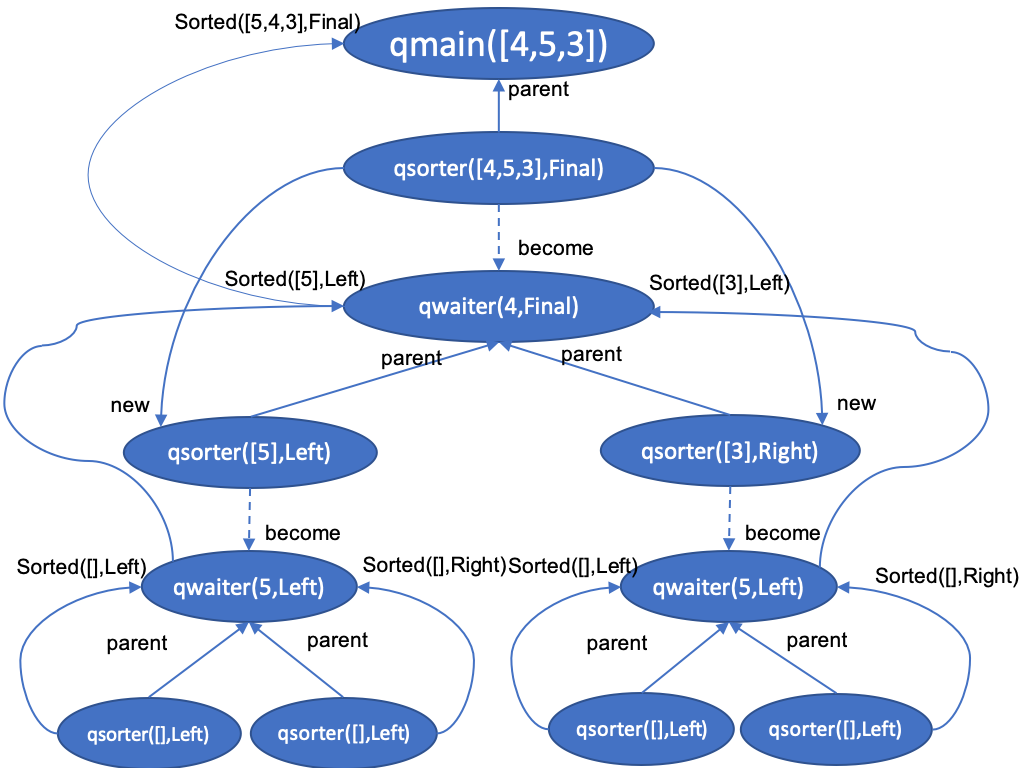
\includegraphics[width=\columnwidth]{qsort}
\caption{Example Quicksort}
\label{fig:example_quicksort}
\end{figure}

Figure \ref{fig:example_quicksort} shows a diagram representation of a simple quicksort in terms of the actors, their links and the messages that are sent. Note the dashed arrow showing \code{qsorter} actors becoming \code{qwaiter} actors.

\subsection{Termites}

\label{subsec:termites}

\begin{figure}
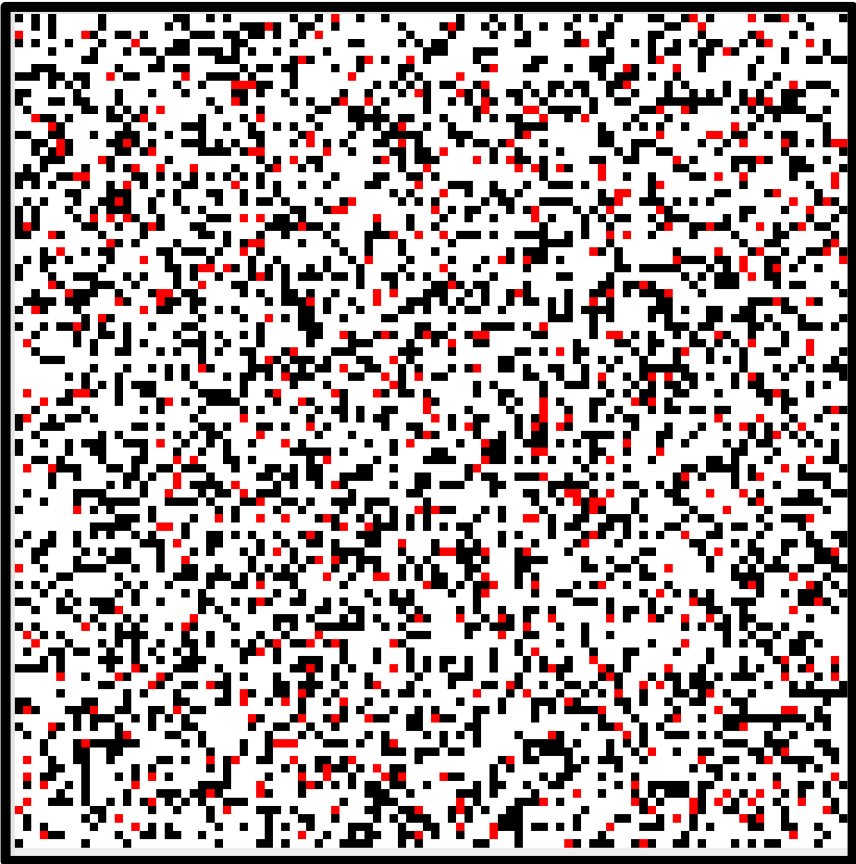
\includegraphics[width=0.4\columnwidth]{termites_before}
\hfill
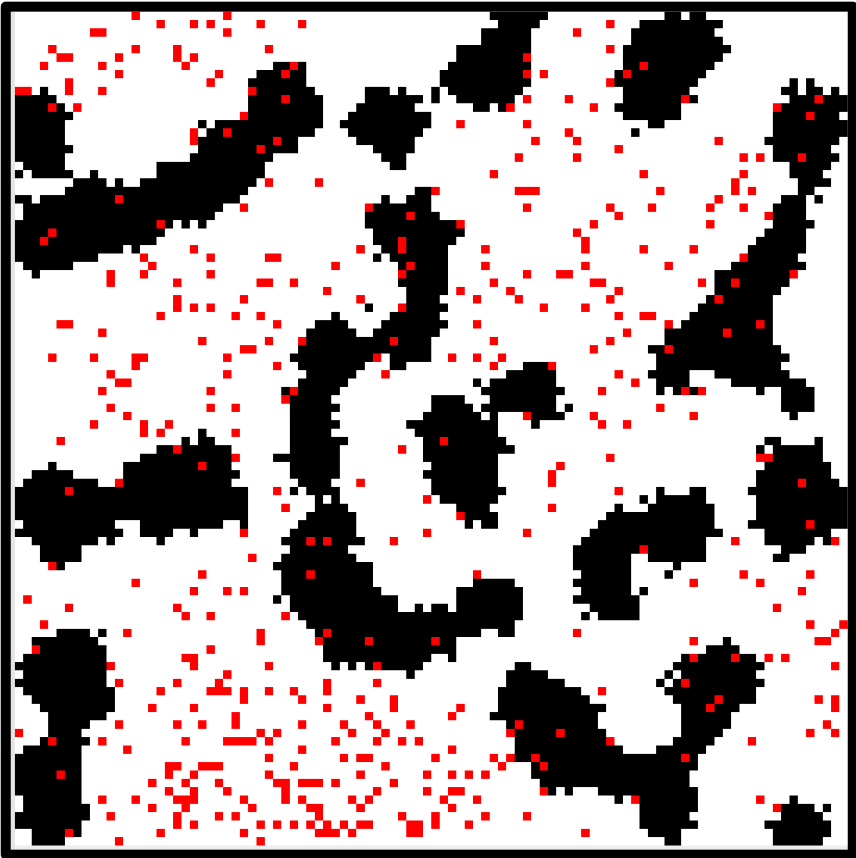
\includegraphics[width=0.41\columnwidth]{termites_after}
\caption{Termites Before and After}
\label{fig:termites}
\end{figure}

Actor based systems can be used to exhibit {\it emergent behaviour} where system-level behaviour can be observed as a result of many simple individual behaviours even though each individual behaviour has no knowledge of the whole. An example is {\it termites} shown in figure \ref{fig:termites} where a collection of twigs (black squares) and moved by a collection of termites (red squares) to form piles even though the individual termites do not have any knowledge of pile-formation.

The behaviour of a termite is simple: walk around at random until a twig is found that is not next to other twigs. The termite then picks up the lone-twig and walks at random until it finds another twig that is next to other twigs. The termite then drops the twig and then starts over again.


\begin{figure*}
\hrule\textwidth1cm
\begin{multicols}{2}
\begin{FigESL}
Act Main { Time(Int); }
Act Grid { SetColour(Int,Int,Str); TermiteAt(Int,Int,Int);}

size::Int          = 120;
limit::Int         = 40000;
numOfTermites::Int = 600;
twig::Str          = 'black';
background::Str    = 'white';
grid::Grid         = new 'esl.grid.Grid'[Grid](size,size,6); 

isLegal(x::Int,y::Int)::Bool = 
  (x >= 0 and x < size) and (y >= 0 and y < size);

Act Termite {  Search; Drop; FindSpace; GetAway(Int); }

act termite(id::Int,w::World)::Termite { 

  x::Int  = random(size);
  y::Int  = random(size);
  dx::Int = random(3) - 1;
  dy::Int = random(3) - 1;
  
  randomDir()::Void = {
    dx := random(3)-1;
    dy := random(3)-1;
  }
  move()::Void = {
    x := (x + dx); y := (y + dy);
    if x < 0 
    then { dx := 1; x := 0; move();
    } else if x > (size - 1)
    then { dx := (0-1); x := (size - 1); move();
    } else if y < 0 
    then { dy := 1; y := 0; move();
    } else if y > (size - 1)
    then { dy := 0 -1; y := (size - 1); move();
    } else grid <- TermiteAt(id,x,y);
  }
  moveRandom()::Void = {
    randomDir();
    move();
  }
  
  -> self <- Search;
  
  Search -> {
    moveRandom();
    w <- TryPickup(x,y,self);
  }
  Drop -> {
    moveRandom();
    w <- FindPile(x,y,self);
  }
  FindSpace -> {
    moveRandom();
    w <- TryDrop(x,y,self);
  }
  GetAway(0) -> {
    self <- Search;
  }
  GetAway(n::Int) -> {
    move();
    self <- GetAway(n-1);
  }
}


Act World {
  TryPickup(Int,Int,Termite);
  FindPile(Int,Int,Termite);
  TryDrop(Int,Int,Termite);
}

act world::World {
  locations::Array[Array[Str]] =
    let a::Array[Array[Str]] = new Array[Array[Str]](size);
    in {
      for x::Int in 0..size do {
        a[x] := new Array[Str](size);
        for y::Int in 0..size do {
          a[x][y] := if random(100) < 30 
                     then twig 
                     else background;
          grid <- SetColour(x,y,a[x][y]);
        }
      }
      edb.display[Grid]('Termites',grid); 
      a;
    }
  termites::[Termite] = 
    [ new termite(n,self) | n::Int <- 0..numOfTermites ];
  foundSingleton(x::Int,y::Int)::Bool = 
    locations[x][y] = twig and twigCount(x,y) < 5;
  foundPile(x::Int,y::Int)::Bool = 
    locations[x][y] = twig and twigCount(x,y) > 4; 
  isTwig(x::Int,y::Int)::Bool =  
    if isLegal(x,y) 
    then locations[x][y] = twig; 
    else false;
  twigCount(x::Int,y::Int)::Int = 
    sum([ if isTwig(x+dx,y+dy) then 1 else 0 | 
          dx <- [-1,0,1], 
          dy <- [-1,0,1], 
          ?(x<>0 or y<>0) ]);
      
  TryPickup(x::Int,y::Int,t::Termite) -> { 
    if foundSingleton(x,y)
    then {
      locations[x][y] := background;
      grid <- SetColour(x,y,background);
      t <- Drop;
    } else t <- Search;
  }
  FindPile(x::Int,y::Int,t::Termite) -> { 
    if foundPile(x,y)
    then t <- FindSpace;
    else t <- Drop;
  }
  TryDrop(x::Int,y::Int,t::Termite) -> {
    if locations[x][y] = background
    then {
      locations[x][y] := twig;
      grid <- SetColour(x,y,twig);
      t <- GetAway(20);
    } else t <- FindSpace;
  }
}

w::World = new world;

act main::Main {
  Time(n::Int) when n > limit -> stopAll();
  Time(n::Int) -> { } 
}
\end{FigESL}
\end{multicols}
\hrule\textwidth1cm\vspace{.5cm}
\caption{Termites}
\label{fig:esl_termites}
\end{figure*}

The implementation of termites in ESL is shown in figure \ref{fig:esl_termites}. The implementation shows a typical scenario in actor-based systems where there is a single world-state and many different actors that share the state. Each individual needs the state in order to determine its next move which involves an update to the world state. Given that all the actors are operating concurrently, this dependency on a single world state can cause problems if access and updates are not protected. Conventional programming languages provide {\it data locks} to deal with shared state. 

ESL provides locks, but often they are not required because actors operate in terms of asynchronous messages and queues. The diagram below shows how this works:
\begin{center}
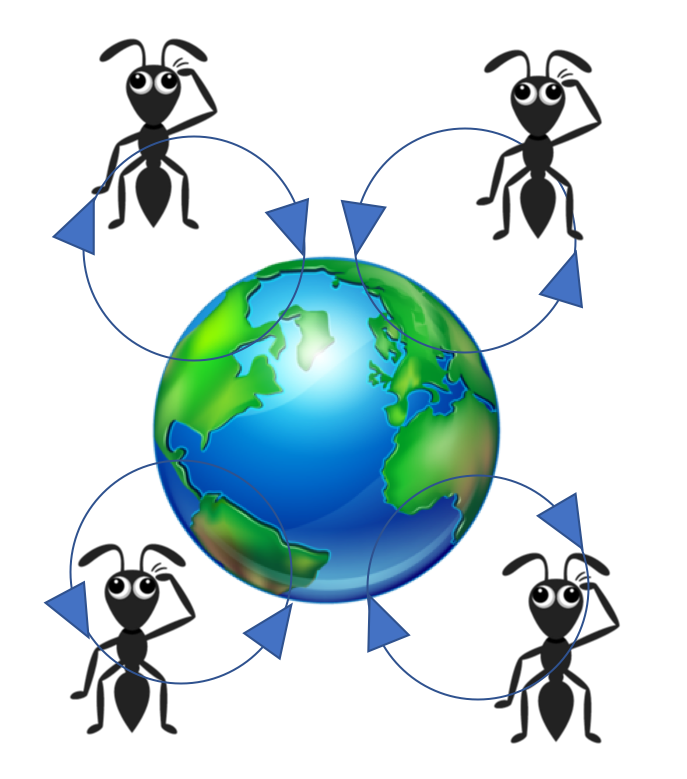
\includegraphics[width=0.5\columnwidth]{termites}
\end{center} 
The world at the centre of the figure represents the shared state. Four independent worker actors are shown, although any number can be involved. The shared state offers an interface that supports the operations required by the worker actors which, in turn, provide an interface that represents the different outcomes from performing the world operations.

From the perspective of a single worker, it looks like they get dedicated access to the shared world state because a message sent to the world is queued until the world becomes free. Each worker message must include the worker actor so that the shared state can reply to it. When a worker sends a message to the shared state the worker becomes idle and will be woken up by the reply from the shared state. When the shared state processes a worker message, the worker has exclusive access to the data, the data can be changed and then the message is sent back to the worker which is woken up.

\subsection{Dining Philosophers}

\label{sec:dining_philosophers}

Dining Philosophers is a standard scenario that is used to exemplify the issues of shared access to resources. Several concurrent processes (philosophers) are vying for shared resources (chopsticks) in order to eat. Each process needs exactly two resources to each and each resource is shared by exactly two processes. When a process acquires a pair of resources, it performs activity (eats) and then releases the resources. Access to resources is assumed to be fair. If a process acquires resources sequentially, then a situation can arise where all resources have acquired one resource and is awaiting on a resource that has been acquired by another process (starvation). In order to avoid starvation, the processes need to wait until they can individually acquire a pair of resources as an atomic action.

A situation where the philosophers are happily eating is shown below:
\begin{center}
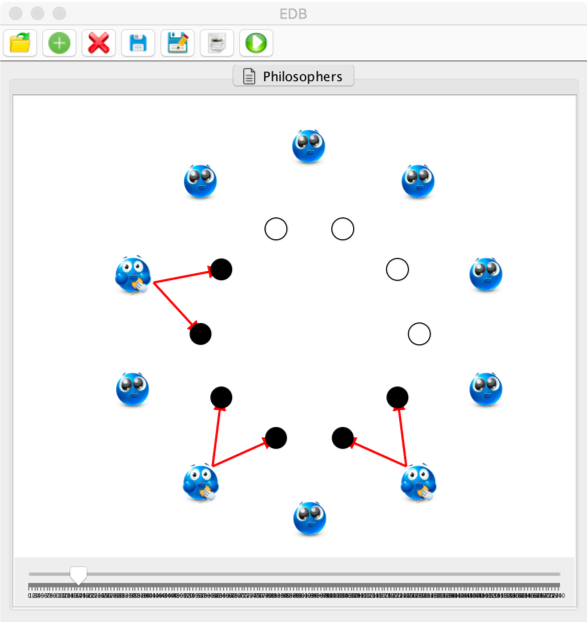
\includegraphics[width=0.49\columnwidth]{dining1}
\hfill
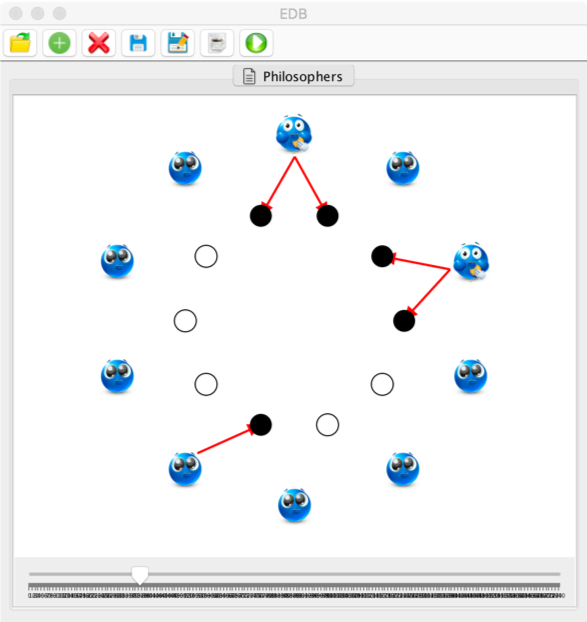
\includegraphics[width=0.49\columnwidth]{dining2}
\end{center}
In the case where chopsticks are grabbed one at a time, the situation rapidly deadlocks:

\begin{center}
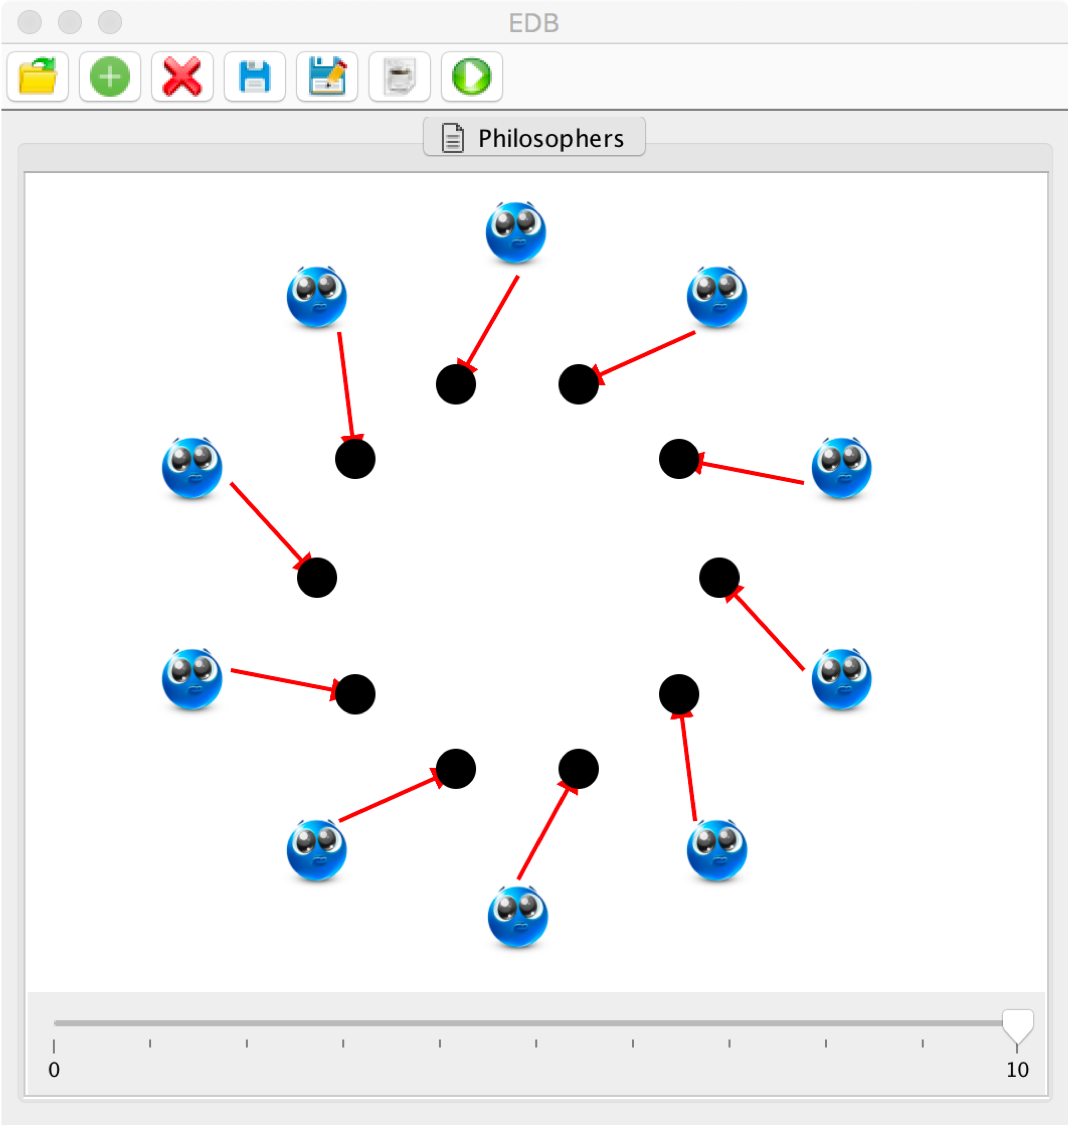
\includegraphics[width=0.49\columnwidth]{dining3}
\end{center}
The implementation of deadlock-free dining philosophers is shown below:
\begin{ESL}
numberOfPhilosophers::Int = 10;    
eatTime::Int              = 50;       
thinkTime::Int            = 50;   

Act Main { Time(Int); }
Act Chopstick { }  
Act Philosopher { Time(Int); }

eat()::Void   = wait(eatTime);
think()::Void = wait(thinkTime);

act philosopher(i::Int,
                left::Chopstick,
                right::Chopstick)::Philosopher {
  Time(n::Int) -> {
    think();
    grab(left,right) {
      eat();
    }  
  }
}

act chopstick::Chopstick {}

chopsticks::[Chopstick] = 
  [ new chopstick | i::Int <- 0..numberOfPhilosophers ];
chop(i::Int)::Chopstick = 
  nth[Chopstick](chopsticks,i%numberOfPhilosophers);

philosophers::[Philosopher] = 
  [ new philosopher(i,chop(i),chop(i+1))
  | i::Int <- 0..numberOfPhilosophers ]; 
\end{ESL}
Deadlock is avoided because the \code{grab} block acquires the locks on \code{left} and \code{right} at the same time. If the locks are not available then the \code{grab} block will wait until they are both free and acquire them simultaneously. Changing the definition of \code{philosopher} to the following leads to deadlock:
\begin{ESL}
act philosopher(i::Int,
                left::Chopstick,
                right::Chopstick)::Philosopher {
  Time(n::Int) -> {
    think();
    grab(left) {
      grab(right) {
        eat();
      }
    }  
  }
}
\end{ESL}

\subsection{Segregation}

\label{sec:segregation}



\section{Polymorphism}

\label{sec:polymorphism}

%%% Map Reduce
%%% Cache

\section{Simulation}

%%% Shop.

\section{Object Orientation}

%%% Subtypes.
%%% Inheritance.
%%% Pacman.

\section{EDB}

\section{Java Interface}

\section{Type Checking}

\section{Compilation}

\section{Implementation}

\bibliography{bibv4}

\clearpage

\appendix

\renewcommand*{\thesection}{\Alph{section}}

\section{Syntax and Type Checking}

\label{sec:syntax}

\begin{figure*}
\begin{tabular}{l|l}
\hline
\begin{minipage}{.275\textwidth}
\footnotesize
{\it Syntax}:\\
\begin{tabular}{llr}
t ::= & & {\it terms}\\
& {\tt x} & {\it variable}\\
& {\tt {\bf new}(t)}& {\it creation}\\
& $\lambda$(\={d}) t&{\it function}\\
& {\tt {\bf act} \{ \={d} \={h} \}}&{\it behaviour}\\
& n & {\it number}\\
& s & {\it string} \\
& b & {\it boolean}\\
& {\bf grab}(x) t & {\it lock}\\
& {\bf if} t {\bf then} t {\bf else} t& {\it conditional}\\
& t $\leftarrow$ t&{\it send}\\
& {\bf case} t \{ \={h} \}&{\it projection}\\
& [\={t}]&{\it list}\\
& t(\={t}) & {\it application}\\
& t[\={T}]& {\it type application}\\
& C(\={t}) & {\it injection}\\
i ::= & d=t& {\it initialisation}\\
d ::= & x[\={X}]::T& {\it declarations}\\
h ::= & C(\={x}) $\rightarrow$ t&{\it handlers}\\
T ::= & & {\it types}\\
& {\bf Int} & {\it integer type}\\
& {\bf Bool} & {\it boolean type}\\
& {\bf Str} & {\it string type}\\
& $\forall$ \={X} . T & {\it universal}\\
& X & {\it variable}\\
& {\bf Union} \{ \={m} \}&{\it union}\\
& {\bf Act} \{ \={d} \={m} \} & {\it behaviour}\\
& (\={T}) $\rightarrow$ T & {\it function type}\\
m ::= & C(\={T}) & {\it message type}\\
\end{tabular}
\end{minipage}
&
\begin{minipage}{0.7\textwidth}
\footnotesize
{\it Type Checking}:\\
\[\begin{array}{cc}
\begin{array}{cr}
\inference{{\tt x::T}\in\Gamma}{\Gamma\vdash{\tt x::T}}&\text{T-VAR}\\\\
\inference{\Gamma\vdash{\tt t}::\text{\tt {\bf Act} \{ \={d} \={m} \}}}{\Gamma\vdash{\tt {\bf new}(t)} :: \text{\tt {\bf Act} \{ \={d} \={m} \}}}&\text{T-NEW}\\\\
\inference{\Gamma,\text{\={x}::\={T}}\vdash\text{t::T}}{\Gamma\vdash\text{$\lambda$(\={d}) t::(\={T})$\rightarrow$T}}&\text{T-FUN}\\\\
%
\Gamma\vdash\text{\tt {\bf act} \{ \={d} \={m} \}::{\bf Act} \{ \={d} \={m} \}}&\text{T-ACT}\\\\
\inference{\Gamma\vdash\text{t\textsubscript{1}::{\bf Act} \{ \={d} \={m} \}}\\\Gamma\vdash\text{t\textsubscript{2}::{\bf Union} \{ \={m} \}}}{\Gamma\vdash\text{t\textsubscript{1}$\leftarrow$ t\textsubscript{2}::{\bf Union} \{ \={m} \}}}&\text{T-SEND}\\\\
%
\Gamma\vdash\text{\tt n::{\bf Int}}&\text{T-INT}\\\\
\Gamma\vdash\text{\tt s::{\bf Str}}&\text{T-STR}\\\\
\Gamma\vdash\text{\tt b::{\bf Int}}&\text{T-BOOL}\\\\
\inference{\Gamma\vdash\text{\tt t::T}}{\Gamma\vdash\text{\tt{\bf grab}(x) t :: T}}&\text{T-LOCK}\\\\
\inference{\Gamma\vdash\text{\tt t\textsubscript{1}::Bool}\\\Gamma\vdash\text{\tt t\textsubscript{2},t\textsubscript{3}::T}}{\Gamma\vdash\text{\tt{\bf if} t\textsubscript{1} {\bf then} t\textsubscript{2} {\bf else} t\textsubscript{3} :: T}}&\text{T-IF}
\end{array}
&
\begin{array}{cr}
\inference{
\Gamma\vdash{\tt {\bf case}\ t\ \{ \text{\={m}}\textsubscript{1} \} :: T}\\
\Gamma\vdash{\tt {\bf case}\ t\ \{ \text{\={m}}\textsubscript{2} \} :: T}}
{
\Gamma\vdash{\tt {\bf case}\ t\ \{ \text{\={m}}\textsubscript{1},\text{\={m}}\textsubscript{2} \} :: T}}&\text{T-CASE1}\\\\
\inference{
\Gamma\vdash{\tt t\textsubscript{1} :: {\bf Union} \{ \text{\={m}},C(\text{\={T}}) \}}\\
\Gamma,{\tt\text{\={x}}::\text{\={T}}\vdash t\textsubscript{2}::T}}{
\Gamma\vdash{\tt {\bf case}\ t\textsubscript{1}\ \{ C(\text{\={x}}) \rightarrow t\textsubscript{2} \} :: T}}&\text{T-CASE2}\\\\
\Gamma\vdash{\tt [] :: \forall X. [X]}&\text{T-NIL}\\\\
\inference{\Gamma\vdash{\tt [\text{\={t}}\textsubscript{1}] :: [T]}\\\Gamma\vdash{\tt [\text{\={t}}\textsubscript{2}] :: [T]}}{
\Gamma\vdash\text{[\={t}\textsubscript{1},\={t}\textsubscript{2}] :: [T]}}&\text{T-LIST1}\\\\
\inference{\Gamma\vdash{\tt t::T}}{\Gamma\vdash{\tt[t]::[T]}}&\text{T-LIST2}\\\\
\inference{\Gamma\vdash{\tt \text{\={t}}::\text{\={T}}}\\\Gamma\vdash{\tt t::(\text{\={T}})\rightarrow T}}{
\Gamma\vdash{\tt t(\text{\={t}})::T}}&\text{T-APP}\\\\
\inference{\Gamma\vdash{\tt t::\forall\text{\={X}}.T}}{\Gamma\vdash{\tt t[\text{\={T}}]::T[\text{\={T}}/\text{\={X}}]}}&\text{T-TAPP}\\\\
\inference{\Gamma,{\tt C(\text{\={T}})}\mapsto{\tt {\bf Union} \{ \text{\={m}} \}}\\
\Gamma\vdash{\tt \text{\={t}}::\text{\={T}}}}{\Gamma\vdash{\tt C(\text{\={t}})::{\bf Union} \{ \text{\={m}} \}}}&\text{\tt T-INJ}\\\\
\end{array}
\end{array}\]
\end{minipage}
\\
\hline
\end{tabular}
\caption{ESL Syntax and Type Checking}
\label{fig:ESL_type_checking}
\end{figure*}

\section{List Operations}

\label{sec:list_operations}


\begin{FigESL}
adjoin[T](x::T,l::[T])::[T] =
  if member[T](x,l)
  then l;
  else x:l;
  
select1[T](l::[T],d::T,p::(T)->Bool)::T =
  case l {
    [] -> d;
    h:t when p(h) -> h;
    h:t -> select1[T](t,d,p);
  }

map[M,N](f::(M)->N,l::[M])::[N] =
  case l {
    [] -> [];
    m:ms -> (f(m)):map[M,N](f,ms); 
  }
  
remove[T](v::T,l::[T])::[T] =
  case l {
    h:t when (h=v) -> remove[T](v,t);
    h:t        -> h:remove[T](v,t);
    []         -> [];
  }

remove1[T](v::T,l::[T])::[T] =
  case l {
    h:t when (h=v) -> t;
    h:t        -> h:remove1[T](v,t);
    []         -> [];
  }

length[T](l::[T])::Int = 
  case l {
    h:t -> 1 + length[T](t);
    [] -> 0;
  }

flatten[T](lists::[[T]])::[T] =
  case lists {
    h:t -> h+flatten[T](t);
    [] -> [];
  }
        
count[T](x::T,l::[T])::Int =
  case l {
    h:t -> if h=x then 1+count[T](x,t); else count[T](x,t);
    []  -> 0;
  }
  
hasPrefix[T](list::[T],prefix::[T])::Bool =
  case list,prefix {
    l1,[] -> true;
    x:list,y:prefix when x=y -> hasPrefix[T](list,prefix);
    l1,l2 -> false;
  }
  
nth[T](l::[T],n::Int)::T =
  case l {
    h:t    -> if n = 0 then h; else nth[T](t,n-1);
    []  -> throw[T]('cannot take nth element.');
  }
  
take[T](l::[T],n::Int)::[T] = 
  if n = 0
  then [];
  else 
    case l {
      h:t -> h:(take[T](t,n-1));
      [] -> throw[[T]]('cannot take element ' + n);
    }
  
drop[T](l::[T],n::Int)::[T] = 
  if n = 0
  then l;
  else 
    case l {
      h:t -> drop[T](t,n-1);
      [] -> throw[[T]]('cannot drop element ' + n);
    }
    
subst[T](n::T,o::T,l::[T])::[T] =
  case l {
    [] -> [];
    h:t -> 
      if h = o 
      then n:(subst[T](n,o,t)); 
      else h:(subst[T](n,o,t));
  }
  
head::Forall[T]([T])->T = fun(l::[T])::T
  case l {
    h:t -> h;
    [] -> throw[T]('cannot take the head of []');
  }
  
tail::Forall[T]([T])->[T] = fun(l::[T])::[T]
  case l {
    h:t -> t;
    [] -> throw[[T]]('cannot take the tail of []');
  }
  
isNil[T](l::[T])::Bool =
  case l {
    [] -> true;
    l -> false;
  }
  
member[T](e::T,l::[T])::Bool =
  case l {
    [] -> false;
    x:xs when x = e -> true;
    x:xs-> member[T](e,xs);
  }
  
reverse[T](l::[T])::[T] =
  case l {
    [] -> [];
    x:xs -> reverse[T](xs) + [x];
  }

exists[T](pred::(T)->Bool,l::[T])::Bool =
  case l {
    [] -> false;
    x:xs when pred(x) -> true;
    x:xs -> exists[T](pred,xs);
  }

forall::[T](pred::(T)->Bool,l::[T])::Bool =
  case l {
    [] -> true;
    x:xs when pred(x) -> forall[T](pred,xs);
    x:xs -> false;
  }
  
replaceNth[T](l::[T],n::Int,x::T)::[T] = 
  case l {
    [] -> throw[[T]]('cannot replace nth of []');
    h:t when n=0 -> x:t;
    h:t -> h:replaceNth[T](t,n-1,x);
  }

indexOf[T](t::T,l::[T])::Int =
  case l {
    [] -> 0-1;
    h:l when h=t -> 0;
    h:l -> 1 + indexOf[T](t,l);
  }
  
select[T](p::(T)->Bool,l::[T])::[T] =
  case l {
    [] -> [];
    h:t when p(h) -> h:select[T](p,t);
    h:t -> select[T](p,t);
  }
  
reject[T](p::(T)->Bool,l::[T])::[T] =
  case l {
    [] -> [][T];
    h:t when p(h) -> reject[T](p,t);
    h:t -> h:reject[T](p,t);
  }
  
last[T](l::[T])::T =
  case l {
    [] -> throw [T]('no last element of empty list');
    x:[] -> x;
    h:l -> last[T](l);
  }
  
butlast[T](l::[T])::[T] =
  case l {
    [] -> [];
    [x] -> [];
    h:l -> h:butlast[T](l);
  }

occurrences[T](x::T,l::[T])::Int =
  case l {
    [][T] -> 0;
    h:t when h=x -> 1 + occurrences[T](x,t);
    h:t -> occurrences[T](x,t);
  }
  
filter[T](pred::(T)->Bool,l::[T])::[T] = 
  case l {
    [] -> [];
    h:t ->
      if pred(h) 
      then h:filter[T](pred,t);
      else filter[T](pred,t);
  }
  
foldr[M,N](map::(M)->N,op::(N,N)->N,empty::N,list::[M])::N =
  case list {
    [] -> empty;
    h:t -> op(map(h),foldr[M,N](map,op,empty,t));
  }
  
id[T]::(T)->T = fun(x::T)::T x;
  
sum(list::[Int])::Int = 
  foldr[Int,Int](id[Int],fun(x::Int,y::Int)::Int x+y,0,list);

removeDups[T](list::[T])::[T] =
  case list {
    [] -> [];
    x:l -> x:removeDups[T](remove[T](x,l));
  }
  
prefixes[T](l::[T])::[[T]] =
  letrec pre(prefixes::[[T]],rest::[T])::[[T]] = 
    if rest = []
    then prefixes;
    else pre(prefixes + [ 
           last[[T]](prefixes)+[head[T](rest)] 
         ],tail[T](rest));
  in pre([[]],l);

takeWhile[T](p::(T)->Bool,l::[T])::[T] =
  case l {
    [] -> [];
    t:l when p(t) -> t:takeWhile[T](p,l);
    t:l -> [];
  }

dropWhile[T](p::(T)->Bool,l::[T])::[T] =
  case l {
    [] -> [];
    t:l when p(t) -> dropWhile[T](p,l);
    l -> l;
  } 
  
removeAll[T](removables::[T],l::[T])::[T] =
  case removables {
    [] -> l;
    t:r -> removeAll[T](r,remove[T](t,l));
  }
\end{FigESL}


\end{document}


